\documentclass[a4paper]{article}
\usepackage{eci289I}
\usepackage[pdftex]{graphicx}
\usepackage{natbib}
\usepackage[labelfont=bf,textfont=sf,labelsep=period]{caption} 
%\RequirePackage{lineno} % for line numbers
\usepackage{listings}
\pdfpagewidth=210 true mm
\pdfpageheight=297 true mm

\renewcommand{\rmdefault}{phv} % Arial
\renewcommand{\sfdefault}{phv} % Arial

\bibpunct{[}{]}{;}{a}{,}{,~}

\pagestyle{IEMSSheadings}

% Text to appear in the header of the pages
\IEMSShead{Chen Peng / MRTA solved by GA }



\title{Multi Robots Task Assignments Problems Solved by Evolutionary Algorithm}

%Authors Names and Affiliations:  Two spaces below the title, 10 pt
%Arial, Upper and Lower Case, underline author presenting
%paper and  provide his/her email address

\author{\underline{Chen Peng}
\address[A1]{\it{Mechanical and Aerospace Engineering Department,
UC, Davis, US (penchen@ucdavis.edu, )}}}

\begin{document}
%\linenumbers

\begin{abstract}
This term paper mainly uses genetic algorithm to solve the multi robots task assignment(MRTA) problems in two situations. We assume that each robot can go directly from one point to another and the distance is just the euclidean distance between two points. One task only needs one robot in one assignment and all tasks need to be visited in one task execution. In the first situation, we have the same amounts of robots as the tasks (m vs m), while in the second condition, we have less robots than tasks. The objective function of both problems is to find the shortest summary distances of all the robots to go over all task points. 
\end{abstract}
\begin{keyword}
MRTA, evolutionary algorithm, TSP, mTSP
\end{keyword}

\maketitle


\section{Introduction}

Multi-robot systems (MRS) are a group of robots that are designed
aiming to perform some collective behavior.One of the most challenging problems of MRS is how to optimally assign a set of robots to a set of tasks in such a way that optimizes the overall system performance subject to a set of constraints.This problem is known as Multi-robot Task Allocation (MRTA) problem \cite{MRTASOFA}. In the first situation, we want to match each robot with one particular task so that the total distance is shortest. This is very similar to the classic problem of traveling salesman problem: "Given a list of cities and the distances between each pair of cities, what is the shortest possible route that visits each city exactly once and returns to the origin city?"\cite{wikiwebTSP} In the second condition, we consider less robots to visit more tasks. This problem is very similar to mTSP problem: The multiple traveling salesman problem (MTSP) involves scheduling m \textless 1 salesmen to visit a set of n \textgreater m nodes so that each node is visited exactly once.\cite{sedighpour2012effective} 

\section{m robots m tasks}
In the first situation, we assume that the robots are just equal to the amount of tasks and we want to choose the optimal task allocations to make minimum the total distances of all the robots will go over. If we solve this problem by exhaustive permutation of all the robots (or tasks), it will be a NP hard problem and the complexity is O(n$!$). Therefore, we need to choose other methods to decrease the computation complexity to make the problem solvable in high dimension.


\subsection{Evolutionary algorithm model}

In the process of finding optimal result, we use the method of Hill-Climbing. This technique is related to gradient ascent, but it does not require you to know the strength of the gradient or even its direction: you just iteratively test new candidate solutions in the region of your current candidate, and adopt the new ones if they’re better. This enables you to climb up the hill until you reach a local optimum.\cite{Luke2013Metaheuristics} At the same time, we also need to try the global random searching to avoid the local optimal. Here we use the method of simulated annealing to sometimes accept worse solutions with a certain probability and this probability decreases over time based on 'initial temperature' and 'cooling schedule'\cite{johnson1989optimization}.


\subsection{Small numbers trial}
To test the convergence effect and speed of our algorithm, we use exhaustive way to obtain the global minimum to testify the convergence of our algorithm.
\begin{center}
	\begin{tabular}[c]{ |c|c|c| } 
		\hline
		Num of pairs & Global minimum & Optimal searched\\
		\hline 
		5   & 23.6015 & 23.6015 \\ \hline 
		8   & 21.781  & 22.1582 \\ \hline
		10  & 37.531  & 37.531  \\ \hline
		12  & 66.469  & 66.73   \\ \hline
	\end{tabular}
\end{center}
We can also visualize the result and show the converging process in Figure \ref{fig1}.
 \begin{figure}[h]
 \centering
 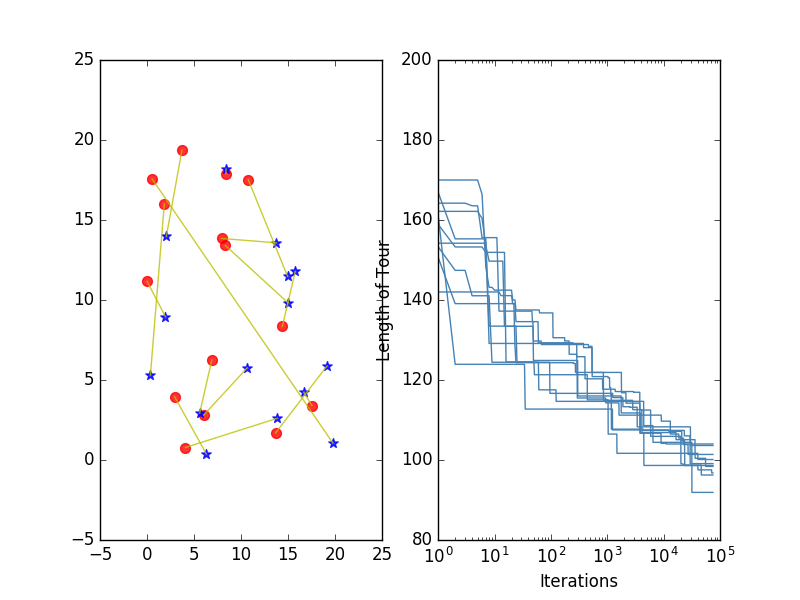
\includegraphics[width=10cm]{Pictures/N10.png}
 \caption{Visualization of task assignment and searching convergence} 
 \label{fig1}
 \end{figure}

\subsection{Large numbers solving}
Photographs should only be used if essential to the clarity of the paper. If used they must be with clear contrast and highly glossed.

\subsection{Complexity of algorithm}
The best upper bound should be very similar to TSP problem. If we set the search range at $[$1,1$]$, then we can use the equation from \cite{steinerberger2015new}. The equation list below:
	\[L =\beta\sqrt{n}\] 
$\beta$ is equal to 0.92



\section{m robots n tasks(m \textless n)}

\subsection{Robot initial alignment}
We can make the initial alignment of the robots to make it as average distributed in the map as possible. In this way, each robot can more likely choose similar amount of tasks and the efficiency of the whole system can be more efficient.
 \begin{figure}[h]
	\centering
	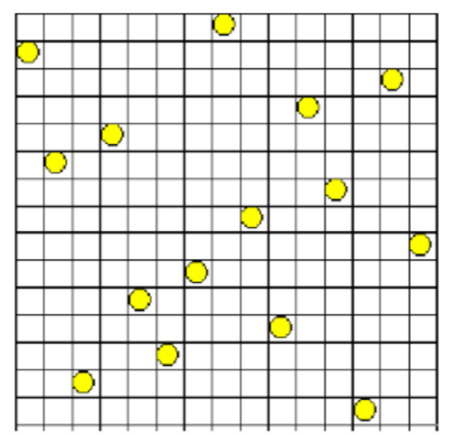
\includegraphics[width=8cm]{Pictures/spacefilling.png}
	\caption{Visualization of task assignment and searching convergence} 
	\label{figspacefilling}
\end{figure}
\subsection{Local search}
At first, we make each task to choose the robot which is nearest to it and then we can obtain the task assignments for each robot. This "Local search" is to meet the requirement that each task is only need one robot to be visited. 
 \begin{figure}[h]
	\centering
	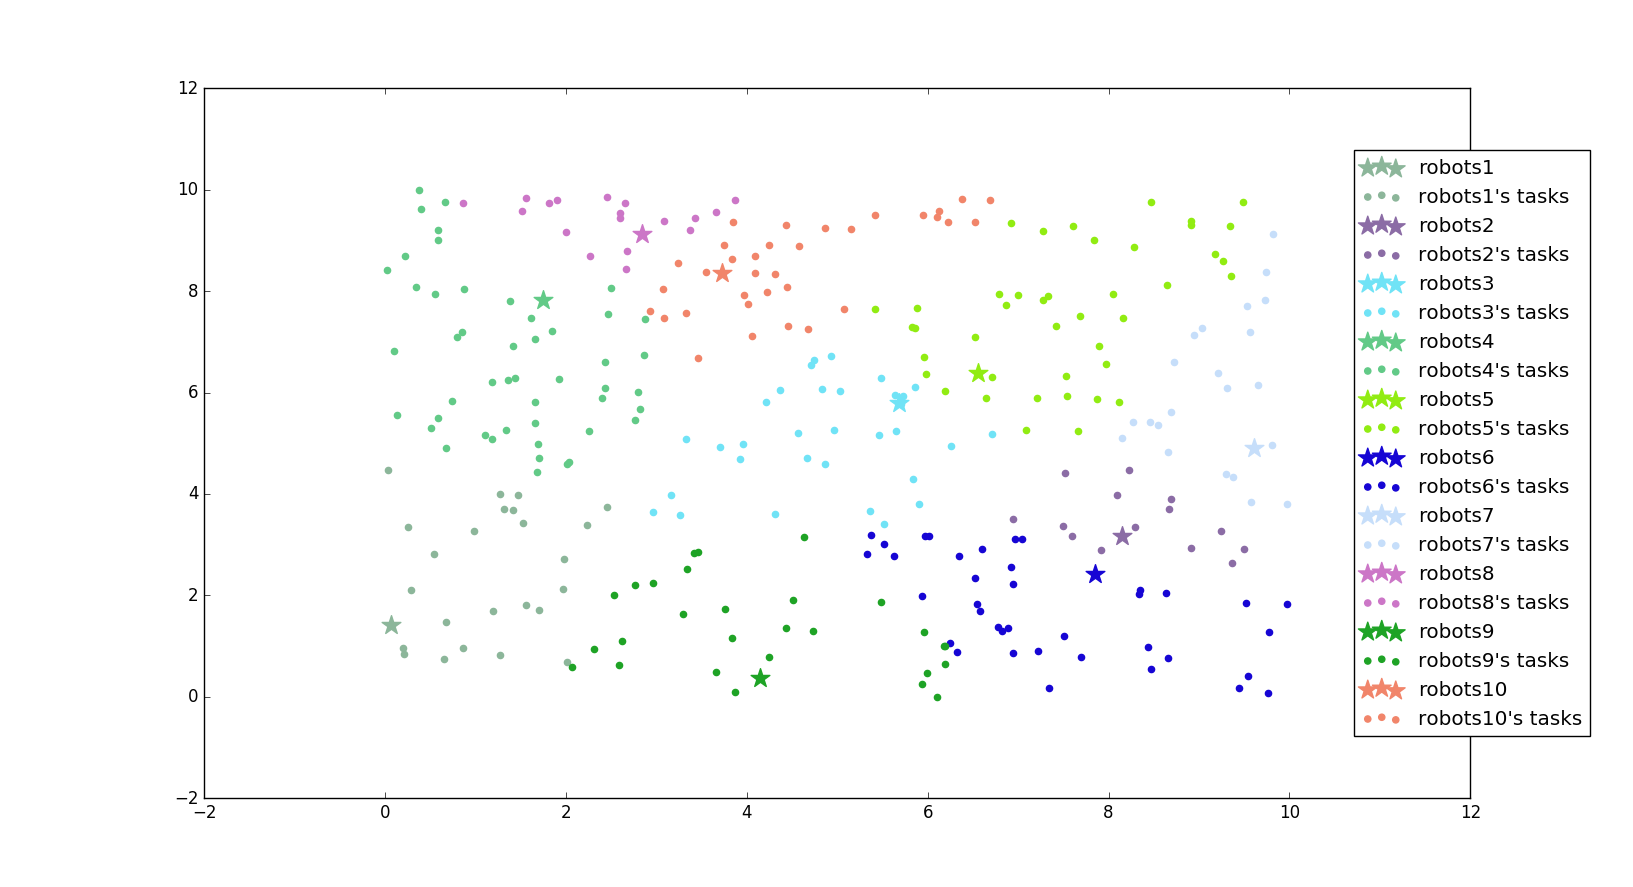
\includegraphics[width=10cm]{Pictures/taskallocation.png}
	\caption{Visualization of task assignment and searching convergence} 
	\label{figtaskallocation}
\end{figure}

\subsection{MRTA solver}
After each robot obtain their task allocation. We can use the TSP method to calculate the minimum distance of each robots will go over their tasks. The result can be visualized in Figure \ref{figtaskexecution}.
 \begin{figure}[h]
	\centering
	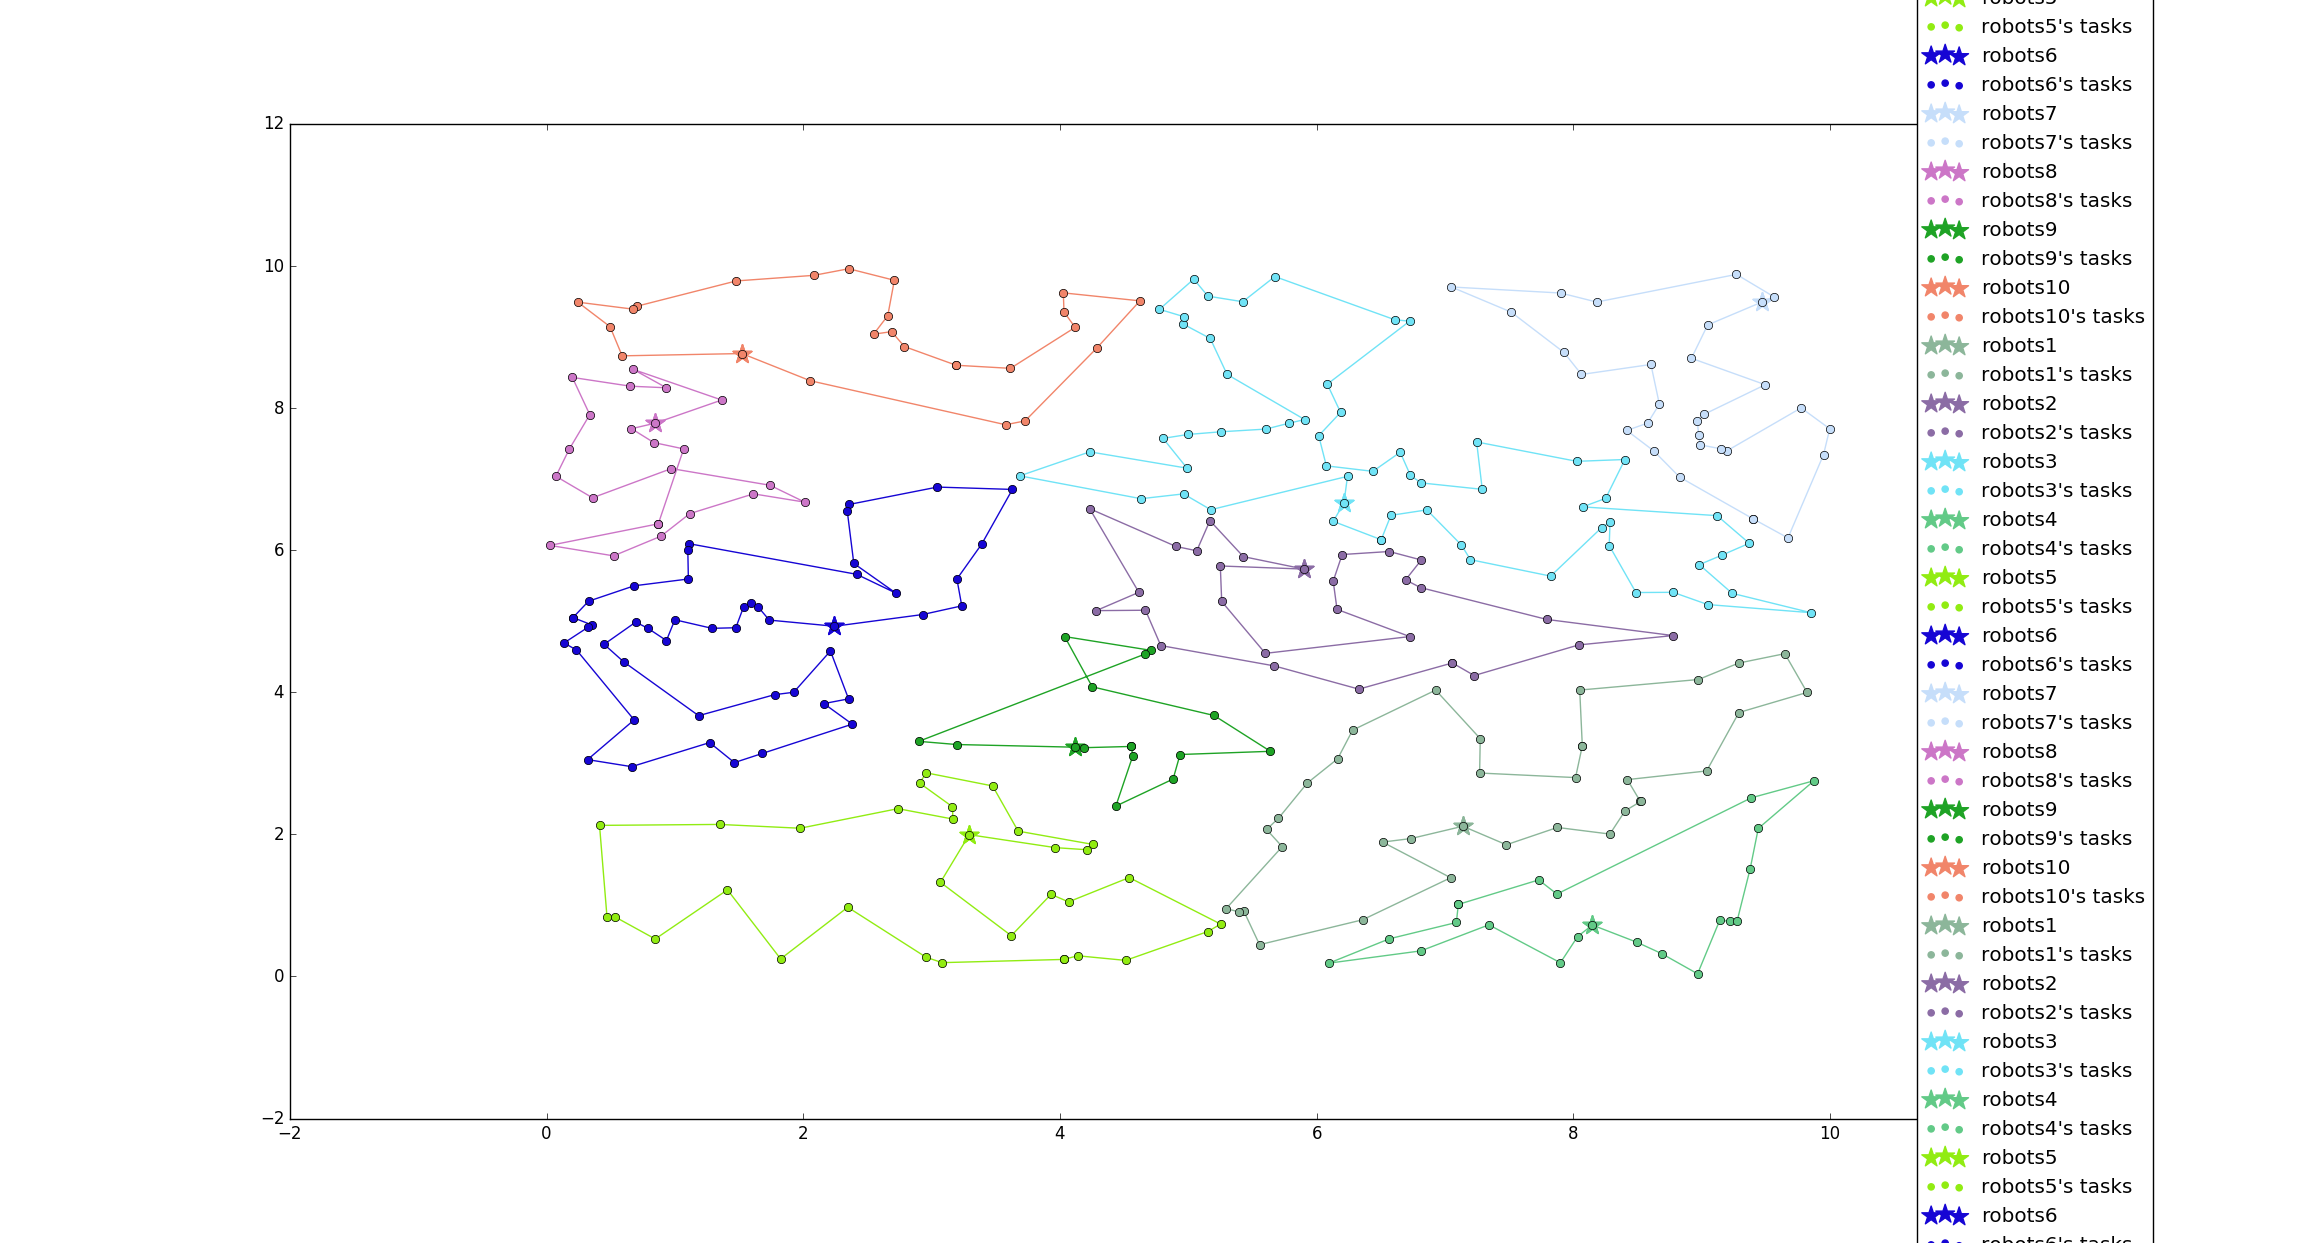
\includegraphics[width=10cm]{Pictures/MRTA.png}
	\caption{Visualization of task assignment and searching convergence} 
	\label{figtaskexecution}
\end{figure}

\section*{Acknowledgments}
This project is advised by Professor Jon Herman and most of the methods I used is from his courses \textbf{ECI 289i}. I very appreciate his great help and awesome course contents in and out of the class. 
%\section*{References}


%%%%%%%%%%%%%%%%%%%%%%%%%%%%%%%%%%%%%%%%%%%%%%%%%%%%%%%%%%%%%%%%%
\bibliographystyle{eci289I}
\bibliography{eci289I-refs}
%%%%%%%%%%%%%%%%%%%%%%%%%%%%%%%%%%%%%%%%%%%%%%%%%%%%%%%%%%%%%%%%%

\section{Appendices}
\subsection{Code of m robots m tasks allocation}
	\lstinputlisting{Codes/MRTA.py}

\subsection{Code of m robots execute n tasks}
\lstinputlisting{Codes/Taskassign.py}

\end{document}
